\documentclass[12pt]{article}
\usepackage{amsmath}
\usepackage{tikz}
\usetikzlibrary{automata, positioning}
\begin{document}

\section*{Defining a Language from a DFA}

To define a language from a given DFA (Deterministic Finite Automaton), you describe the set of strings that the DFA accepts. Here's a step-by-step guide:

\subsection*{1. Describe the DFA}
A DFA is typically defined by a 5-tuple \( M = (Q, \Sigma, \delta, q_0, F) \), where:

\begin{itemize}
    \item \( Q \): A finite set of states.
    \item \( \Sigma \): The input alphabet (a finite set of symbols).
    \item \( \delta \): The transition function \( \delta: Q \times \Sigma \rightarrow Q \), which determines the state transitions based on the current state and input symbol.
    \item \( q_0 \): The start state, where \( q_0 \in Q \).
    \item \( F \): The set of accept (final) states, where \( F \subseteq Q \).
\end{itemize}

\subsection*{2. Define the Language \( L(M) \)}
The language recognized (accepted) by the DFA \( M \), denoted as \( L(M) \), is the set of all strings over the alphabet \( \Sigma \) that the DFA accepts.

Formally, \( L(M) \) is defined as:

\[
L(M) = \{ w \in \Sigma^* \mid \hat{\delta}(q_0, w) \in F \}
\]

where:

\begin{itemize}
    \item \( w \) is a string over the alphabet \( \Sigma \).
    \item \( \Sigma^* \) is the set of all strings (including the empty string) over the alphabet \( \Sigma \).
    \item \( \hat{\delta} \) is the extended transition function, which is recursively defined as:
    \begin{align*}
    \hat{\delta}(q, \epsilon) &= q &\text{(for the empty string \( \epsilon \))} \\
    \hat{\delta}(q, aw) &= \delta(\hat{\delta}(q, a), w) &\text{(for \( a \in \Sigma \) and \( w \in \Sigma^* \))}
    \end{align*}
\end{itemize}

\subsection*{3. Interpretation}
\begin{itemize}
    \item The language \( L(M) \) consists of all strings that, when processed by the DFA starting from the start state \( q_0 \), lead to one of the accept states in \( F \).
    \item If a string \( w \) is in \( L(M) \), the DFA can process \( w \) and end in an accept state.
    \item If a string \( w \) is not in \( L(M) \), the DFA either ends in a non-accepting state or cannot process the string according to its transition rules.
\end{itemize}

\subsection*{Example}

Consider a DFA \( M = (Q, \Sigma, \delta, q_0, F) \) with:

\begin{itemize}
    \item \( Q = \{q_0, q_1, q_2\} \)
    \item \( \Sigma = \{0, 1\} \)
    \item \( \delta \) defined as:
    \begin{align*}
    \delta(q_0, 0) &= q_0 \\
    \delta(q_0, 1) &= q_1 \\
    \delta(q_1, 0) &= q_2 \\
    \delta(q_1, 1) &= q_0 \\
    \delta(q_2, 0) &= q_1 \\
    \delta(q_2, 1) &= q_2
    \end{align*}
    \item \( q_0 \) is the start state.
    \item \( F = \{q_2\} \).
\end{itemize}

\textbf{Language \( L(M) \)}:
\begin{itemize}
    \item The DFA accepts a string if it ends in state \( q_2 \).
    \item \( L(M) \) is the set of strings over \( \{0, 1\} \) that result in the DFA being in state \( q_2 \) after reading the entire string.
\end{itemize}

\subsection*{Conclusion}
To define a language from a DFA, you describe the set of all strings that the DFA accepts. This set is the language recognized by the DFA, and it is formally defined using the extended transition function \( \hat{\delta} \) that describes how the DFA processes each string.

\title{Finite Automata: Language Accepted by DFA}
\author{}
\date{}
\maketitle

\section*{Contents}
Here we are going to formally define what is meant by a DFA (Deterministic Finite Automaton) accepting a string or a language.

\subsection*{Acceptance of a String by a DFA}
A string \( w \) is accepted by a DFA \( M = \langle Q, \Sigma, q_0, \delta, A \rangle \) if and only if \( \hat{\delta}(q_0, w) \in A \). That is, a string is accepted by a DFA if and only if the DFA starting at the initial state ends in an accepting state after reading the string.

\subsection*{Acceptance of a Language by a DFA}
A language \( L \) is accepted by a DFA \( M = \langle Q, \Sigma, q_0, \delta, A \rangle \) if and only if 
\[ 
L = \{ w \mid \hat{\delta}(q_0, w) \in A \} 
\]
That is, the language accepted by a DFA is the set of strings accepted by the DFA.

\section*{Examples}
\newpage
\subsection*{Example 1}
\begin{center}
    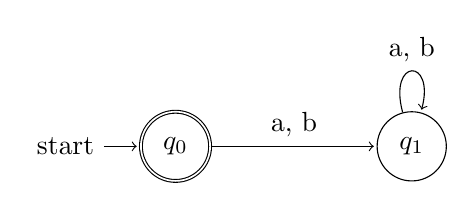
\begin{tikzpicture}[shorten >=1pt, node distance=3cm, on grid, auto]
        % Define the nodes
        \node[state, initial, accepting] (q_0)   {$q_0$}; 
        \node[state] (q_1) [right=of q_0] {$q_1$}; 
     
        % Define the transitions
        \path[->] 
        (q_0) edge[above] node {a, b} (q_1)
        (q_1) edge[loop above] node {a, b} ();
    \end{tikzpicture}
    \end{center}


This DFA accepts \(\{\epsilon\}\) because it can go from the initial state to the accepting state (also the initial state) without reading any symbol of the alphabet, i.e., by reading an empty string \( \epsilon \). It accepts nothing else because any non-empty symbol would take it to state 1, which is not an accepting state, and it stays there.
\newpage
\subsection*{Example 2}
\begin{center}
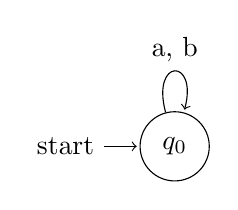
\begin{tikzpicture}[shorten >=1pt, node distance=3cm, on grid, auto]
    \node[state, initial] (q_0)   {$q_0$}; 

    \path[->] 
    (q_0) edge[loop above] node {a, b} (q_0);
\end{tikzpicture}
\end{center}

This DFA does not accept any string because it has no accepting state. Thus, the language it accepts is the empty set \( \emptyset \).
\newpage
\subsection*{Example 3: DFA with One Cycle}
\begin{center}
\begin{tikzpicture}[shorten >=1pt, node distance=3cm, on grid, auto]
    \node[state, initial] (q_0) {$q_0$}; 
    \node[state] (q_1) [right=of q_0] {$q_1$}; 
    \node[state] (q_2) [right=of q_1] {$q_2$}; 
    \node[state, accepting] (q_3) [right=of q_2] {$q_3$}; 
    \node[state] (q_4) [below=of q_1] {$q_4$}; 
    
    \path[->] 
    (q_0) edge[above] node {a} (q_1)
    (q_0) edge[below] node {b} (q_4)
    (q_1) edge[bend left, above] node {a} (q_2)
    (q_2) edge[bend left, below] node {b} (q_1)
    (q_1) edge[right] node {b} (q_4)
    (q_2) edge[above] node {a} (q_3)
    (q_3) edge[right] node {a, b} (q_4)
    (q_4) edge[loop below] node {a, b} ();

\end{tikzpicture}
\end{center}

This DFA has a cycle: 1 - 2 - 1, and it can go through this cycle any number of times by reading the substring "ab" repeatedly.

To find the language it accepts:
\begin{itemize}
    \item First, from the initial state go to state 1 by reading one "a".
    \item Then from state 1, go through the cycle 1 - 2 - 1 any number of times by reading the substring "ab" any number of times to come back to state 1. This is represented by \( (ab)^* \).
    \item Finally, from state 1 go to state 2 and then to state 3 by reading "aa".
\end{itemize}
Thus, a string that is accepted by this DFA can be represented by \( a(ab)^*aa \).
\newpage
\subsection*{Example 4: DFA with Two Independent Cycles}

\begin{center}
    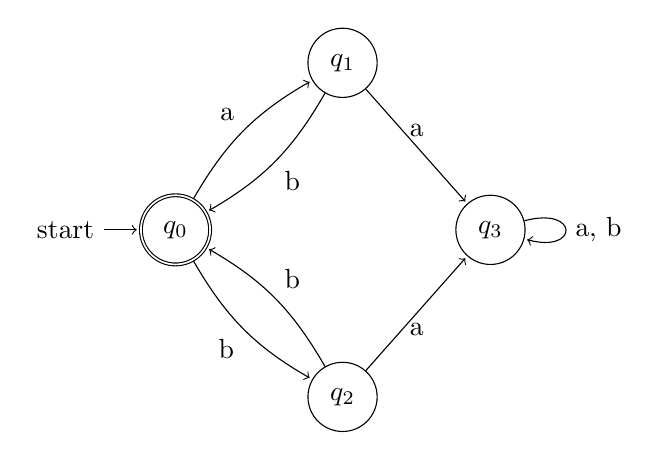
\begin{tikzpicture}[shorten >=1pt, node distance=3cm, on grid, auto]
        % Define the nodes
        \node[state, initial, accepting] (q_0) {$q_0$}; 
        \node[state] (q_1) [above right=of q_0] {$q_1$}; 
        \node[state] (q_2) [below right=of q_0] {$q_2$}; 
        \node[state] (q_3) [right= 4cm of q_0] {$q_3$}; 
        
        % Define the transitions
        \path[->] 
        (q_0) edge[bend left=15, above left] node {a} (q_1)
        (q_0) edge[bend right=15, below left] node {b} (q_2)
        (q_1) edge[bend left=15, below right] node {b} (q_0)
        (q_2) edge[bend right=15, above right] node {b} (q_0)
        (q_1) edge[above] node {a} (q_3)
        (q_2) edge[below] node {a} (q_3)
        (q_3) edge[loop right] node {a, b} ();
    
    \end{tikzpicture}
\end{center}
This DFA has two independent cycles: 0 - 1 - 0 and 0 - 2 - 0, and it can move through these cycles any number of times in any order to reach the accepting state from the initial state, such as 0 - 1 - 0 - 2 - 0 - 2 - 0. Thus, a string that is accepted by this DFA can be represented by \( (ab + bb)^* \).
\newpage
\subsection*{Example 5: DFA with Two Interleaved Cycles}
\begin{center}
    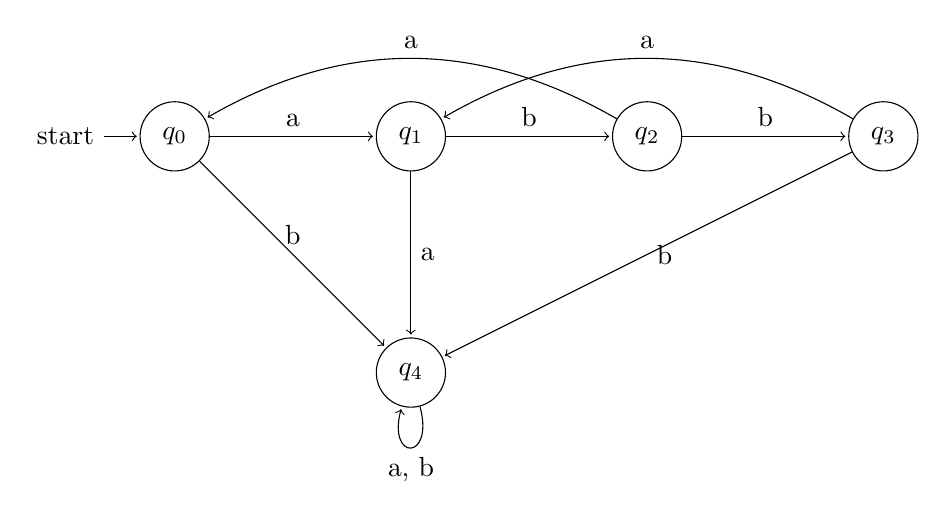
\begin{tikzpicture}[shorten >=1pt, node distance=3cm, on grid, auto]
        % Define the nodes
        \node[state, initial] (q_0) {$q_0$}; 
        \node[state] (q_1) [right=of q_0] {$q_1$}; 
        \node[state] (q_2) [right=of q_1] {$q_2$}; 
        \node[state] (q_3) [right=of q_2] {$q_3$}; 
        \node[state] (q_4) [below=of q_1] {$q_4$};
        % Define the transitions
        \path[->] 
        (q_0) edge[above] node {a} (q_1)
        (q_0) edge[above] node {b} (q_4)
        (q_1) edge[right] node {a} (q_4)
        (q_1) edge[above] node {b} (q_2)
        (q_2) edge[above] node {b} (q_3)
        (q_2) edge[bend right, above] node {a} (q_0)
        (q_3) edge[bend right, above] node {a} (q_1)
        (q_3) edge[right] node {b} (q_4)
        (q_4) edge[loop below] node {a, b} ();

    \end{tikzpicture}
\end{center}
This DFA has two cycles: 1 - 2 - 0 - 1 and 1 - 2 - 3 - 1.

To find the language accepted by this DFA:
\begin{itemize}
    \item First, from state 0 go to state 1 by reading "a". (Any other state which is common to these cycles such as state 2 can also be used instead of state 1).
    \item Then from state 1, go through the two cycles 1 - 2 - 0 - 1 and 1 - 2 - 3 - 1 any number of times in any order by reading substrings "baa" and "bba", respectively. At this point, a substring \( a(baa + bba)^* \) will have been read.
    \item Then go from state 1 to state 2 and then to state 3 by reading "bb".
\end{itemize}
Thus, altogether \( a(baa + bba)^*bb \) will have been read when state 3 is reached from state 0.
\newpage
\subsection*{Example 6}
\begin{center}
    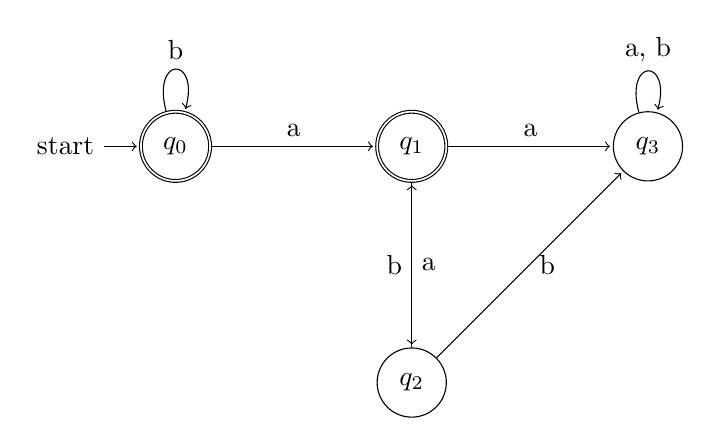
\begin{tikzpicture}[shorten >=1pt, node distance=3cm, on grid, auto]
        % Define the nodes
        \node[state, initial, accepting] (q_0) {$q_0$}; 
        \node[state, accepting] (q_1) [right=of q_0] {$q_1$}; 
        \node[state] (q_2) [below=of q_1] {$q_2$}; 
        \node[state] (q_3) [right=of q_1] {$q_3$}; 
        % Define the transitions
        \path[->] 
        (q_0) edge[loop above] node {b} ()
        (q_0) edge[above] node {a} (q_1)
        (q_1) edge[left] node {b} (q_2)
        (q_1) edge[above] node {a} (q_3)
        (q_2) edge[right] node {a} (q_1)
        (q_2) edge[right] node {b} (q_3)
        (q_3) edge[loop above] node {a, b} ();
    \end{tikzpicture}
\end{center}
This DFA has two accepting states: 0 and 1. Thus, the language that is accepted by this DFA is the union of the language accepted at state 0 and the one accepted at state 1.
\begin{itemize}
    \item The language accepted at state 0 is \( b^* \).
    \item To find the language accepted at state 1, first at state 0 read any number of "b"s. Then go to state 1 by reading one "a". At this point \( (b^*a) \) will have been read. At state 1, go through the cycle 1 - 2 - 1 any number of times by reading the substring "ba" repeatedly. Thus, the language accepted at state 1 is \( b^*a(ba)^* \).
\end{itemize}
\subsection*{More examples}
\begin{center}
    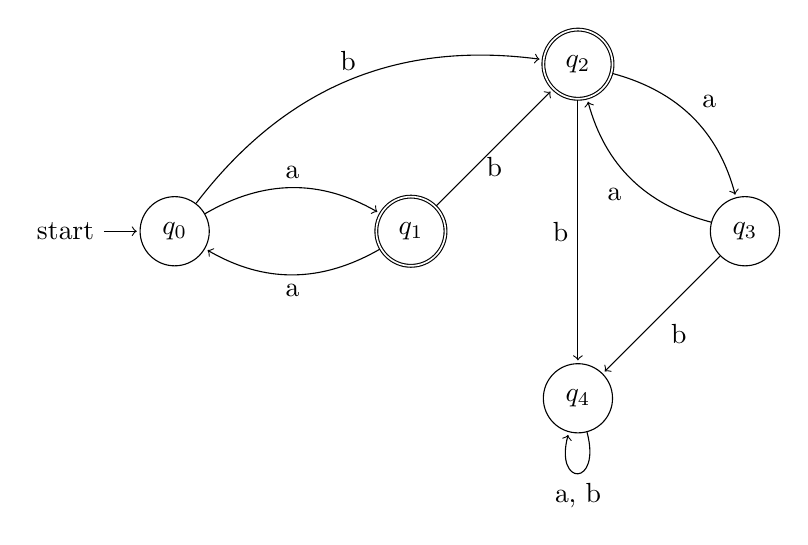
\begin{tikzpicture}[shorten >=1pt, node distance=3cm, on grid, auto]
        % Define the nodes
        \node[state, initial] (q_0) {$q_0$}; 
        \node[state, accepting] (q_1) [right=of q_0] {$q_1$}; 
        \node[state, accepting] (q_2) [above right=of q_1] {$q_2$}; 
        \node[state] (q_3) [below right=of q_2] {$q_3$};
        \node[state] (q_4) [below right=of q_1] {$q_4$};
        % Define the transitions
        \path[->] 
        (q_0) edge[bend left, above] node {a} (q_1)
        (q_0) edge[bend left, above] node {b} (q_2)
        (q_1) edge[bend left, below] node {a} (q_0)
        (q_1) edge[below] node {b} (q_2)
        (q_2) edge[bend left, above right] node {a} (q_3)
        (q_2) edge[left] node {b} (q_4)
        (q_3) edge[bend left, below left] node {a} (q_2)
        (q_3) edge[below right] node {b} (q_4)
        (q_4) edge[loop below] node {a, b} ();
    \end{tikzpicture}
\end{center}
This DFA contains 2 accepting states, suggesting the union of the language accepted at state 1 and state 2.

This DFA also contains 2 separated cycles, 

\end{document}